%%%%%%%%%%%%%%%%%%%%%%%%%%%%%%%%%%%%%%%%%
% Quiz #1 Template
% LaTeX Template
% By: Ryan Grove
%%%%%%%%%%%%%%%%%%%%%%%%%%%%%%%%%%%%%%%%%

%----------------------------------------------------------------------------------------
%	PACKAGES AND OTHER DOCUMENT CONFIGURATIONS
%----------------------------------------------------------------------------------------

\documentclass[paper=a4, fontsize=11pt]{scrartcl} % A4 paper and 11pt font size

\usepackage[T1]{fontenc} % Use 8-bit encoding that has 256 glyphs
\usepackage{fourier} % Use the Adobe Utopia font for the document - comment this line to return to the LaTeX default
\usepackage[english]{babel} % English language/hyphenation
\usepackage{amsmath,amsfonts,amsthm} % Math packages

\usepackage{lipsum} % Used for inserting dummy 'Lorem ipsum' text into the template

\usepackage{sectsty} % Allows customizing section commands
\allsectionsfont{\centering \normalfont\scshape} % Make all sections centered, the default font and small caps

\usepackage{fancyhdr} % Custom headers and footers
\pagestyle{fancyplain} % Makes all pages in the document conform to the custom headers and footers
\fancyhead{} % No page header - if you want one, create it in the same way as the footers below
\fancyfoot[L]{} % Empty left footer
\fancyfoot[C]{} % Empty center footer
%\fancyfoot[R]{\thepage} % Page numbering for right footer
\renewcommand{\headrulewidth}{0pt} % Remove header underlines
\renewcommand{\footrulewidth}{0pt} % Remove footer underlines
\setlength{\headheight}{13.6pt} % Customize the height of the header

\numberwithin{equation}{section} % Number equations within sections (i.e. 1.1, 1.2, 2.1, 2.2 instead of 1, 2, 3, 4)
\numberwithin{figure}{section} % Number figures within sections (i.e. 1.1, 1.2, 2.1, 2.2 instead of 1, 2, 3, 4)
\numberwithin{table}{section} % Number tables within sections (i.e. 1.1, 1.2, 2.1, 2.2 instead of 1, 2, 3, 4)

\setlength\parindent{0pt} % Removes all indentation from paragraphs - comment this line for an assignment with lots of text

\usepackage{lastpage}
\usepackage{fancyhdr}
\cfoot{\thepage\ of \pageref{LastPage}}

\def\v{\hbox{$\mathbf v$}}
\def\w{\hbox{$\mathbf w$}}
\def\u{\hbox{$\mathbf u$}}
\def\x{\hbox{$\textbf{x}$}}
\def\z{\hbox{$\mathbf z$}}
\def\a{\hbox{$\mathbf a$}}
\def\b{\hbox{$\mathbf b$}}
\def\L{\hbox{$\mathcal L$}}
\def\C{\hbox{$\mathbb C$}}
\def\B{\hbox{$\mathcal B$}}
\def\R{\hbox{$\mathbb R$}}
\def\X{\hbox{$\underline X$}}
\def\Q{\hbox{$\mathbb Q$}}
\def\R{\hbox{$\mathbb R$}}
\def\N{\hbox{$\mathbb N$}}
\def\C{\hbox{$\mathbb C$}}
\def\0{\hbox{$\mathbf 0$}}
\def\Y{\hbox{$\underline Y$}}
\def\a{\hbox{$\mathbf a$}}
\def\u{\hbox{$\mathbf u$}}
\def\w{\hbox{$\mathbf w$}}
\def\y{\hbox{$\mathbf y$}}
\def\X{\hbox{$\underline X$}}
\def\dd{\hbox{$\partial $}}
\def\B{\hbox{$\mathcal B$}}
\def\F{\hbox{$\mathcal F$}}
\def\L{\hbox{$\mathcal L$}}
\def\M{\hbox{$\mathcal M$}}
\def\D{\hbox{$\mathscr {D}$}}
\def\RR{\hbox{$\mathscr{R}$}}
\def\I{\hbox{$\mathcal I$}}

\usepackage{amssymb}
%\theoremstyle{plain}
\usepackage[margin = .75in]{geometry}
\newtheorem{claim}{Claim}
\newtheorem{theorem}{Theorem}[section]
\newtheorem{lemma}[theorem]{Lemma}
\newtheorem{proposition}[theorem]{Proposition}
\newtheorem{corollary}[theorem]{Corollary}
\newtheorem{problem}[theorem]{Problem}
%\theoremstyle{definition}
\newtheorem{definition}[theorem]{Definition}
%\theoremstyle{remark}
\newtheorem{remark}[theorem]{Remark}
\newtheorem{remarks}[theorem]{Remarks}
\newtheorem{example}[theorem]{Example}
\newcommand{\ds}{\displaystyle}
\newcommand{\ZZ}{\mathbb{Z}}
\newcommand{\QQ}{\mathbb{Q}}
\newcommand{\e}{\varepsilon}
\newcommand{\bbf}{\textbf}
\newcommand{\p}{\parallel}
\usepackage{color}
\newcommand{\field}[1]{\mathbb{#1}}
\usepackage{amsmath}
\usepackage{amsthm}
\usepackage{amssymb}
\usepackage{mathrsfs}
\usepackage{cancel}
\usepackage{upgreek}
\usepackage{graphicx}
\usepackage{multirow}
\usepackage{setspace}
\usepackage{url}
\usepackage{subfigure}
\usepackage{enumerate}
\usepackage{cases}
\usepackage{mathrsfs}
\usepackage{rotating}

%----------------------------------------------------------------------------------------
%	TITLE SECTION
%----------------------------------------------------------------------------------------

\newcommand{\horrule}[1]{\rule{\linewidth}{#1}} % Create horizontal rule command with 1 argument of height

\title{	
\normalfont \normalsize 
\textsc{Ryan Grove, Clemson University, MATH1080 - 9} \\ [25pt] % Your name, university, class
\horrule{0.5pt} \\[0.4cm] % Thin top horizontal rule
\huge Section 6.1: Area Between Curves \\ % The assignment title
\horrule{2pt} \\[0.5cm] % Thick bottom horizontal rule
}

\author{Date:} % The due date

\date{\normalsize January 11, 2016} % A custom date

\begin{document}

\maketitle % Print the title

\begin{flushleft}
\begin{tabular}{l l}
Name: \rule{3.2in}{.01cm}  & {}%Table number: \rule{1in}{.01cm}\\
\end{tabular}
\end{flushleft}

%----------------------------------------------------------------------------------------
%	Lecture
%----------------------------------------------------------------------------------------

\section*{\textbf{Lecture:}}

Consider the region $S$ that lies between two curves $y=f(x)$ and $y=g(x)$ and between the vertical lines $x=a$ and $x=b$, where $f$ and $g$ are continuous functions and $f(x)\geq g(x)$ for all $x$ in $[a,b]$.

\[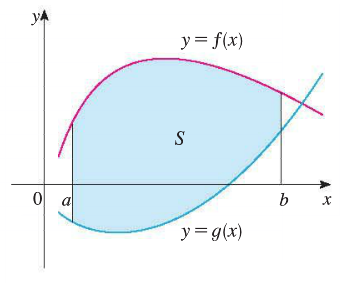
\includegraphics[scale=0.45]{6-1-pic1.png}\]

\fbox{
  \parbox{\textwidth}{
  \vspace{5pt}
  
  \label{1} (1) The area $A$ of the region bounded by the curves $y=f(x)$, $y=g(x)$, and the lines $x=a$, $x=b$, where $f$ and $g$ are continuous and $f(x)\geq g(x)$ for all $x$ in $[a,b]$, is\\
  \indent
  
  \[\underline{\hspace{2in}}\]
  \indent
  
  }}
  \indent\\
  \indent
  
  In the case where both $f$ and $g$ are positive, we can clearly see why (1) is true:
  \[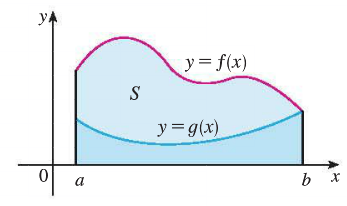
\includegraphics[scale=.45]{6-1-pic2.png}\]
  \begin{align*}
  A &= [\text{area under $y=f(x)$}] - [\text{area under $y=g(x)$}]\\
  &\text{ }\\
  &=\\
  &\text{ }\\
  &= \\
  \end{align*}
  \indent\\
  \indent
  
  \textbf{Note}: If $f$ is positive and $g$ is negative the formula remains the same for then $\ds\int_a^b g(x)dx <0$ so subtracting this negative quantity actually results in adding the area below the x-axis to the area under the graph of $f$ (above the x-axis).\\
  \indent\\
  
  
  \underline{Example 1}: Find the area of the region bounded above by $y=e^x$ , bounded below by $y=x$, and bounded on the sides by $x=0$ and $x=1$.\\
  
  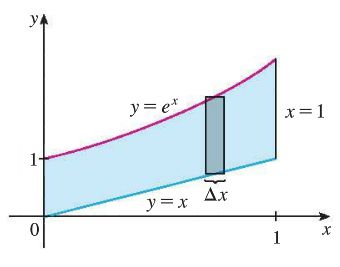
\includegraphics[scale=0.45]{6-1-pic3.png}\\
  \indent\\
  
  \vspace{1.5in}
  
  
  \underline{Example 2}: Find the area of the region enclosed by the parabolas $y=x^2$ and $y=2x-x^2$.\\
  
  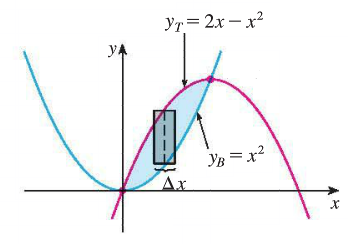
\includegraphics[scale=0.45]{6-1-pic4.png}\\
  \indent\\
  
  \vspace{2.8in}
  
  \textbf{Note:} Sometimes it's difficult, or even impossible, to find the points of intersection of two curves exactly. In this case, a graphing calculator or computer could be used to find approximate values for the intersection points.\\
  \indent
  
  If we are asked to find the area between the curves $y=f(x)$ and $y=g(x)$ where $f(x)\geq g(x)$ for some values of $x$ but $g(x)\geq f(x)$ for other values of $x$, then we split the given region $S$ into multiple regions $S_1,S_2,\ldots$ with areas $A_1,A_2,\ldots$ as shown here:\\
  \[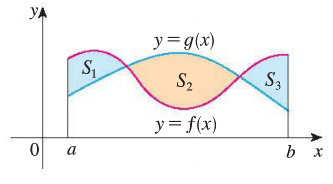
\includegraphics[scale=0.45]{6-1-pic6.png}\]
  We then define the area of the region $S$ to be the sum of the areas of the smaller regions. That is, $A=A_1 + A_2 + \cdots$. Since
  \[|f(x)-g(x)| = \begin{cases}
  f(x) - g(x) &\text{ when } f(x) \geq g(x)\\
  g(x) - f(x) &\text{ when } g(x) \geq f(x)
  \end{cases}\]
  we have the following general expression for $A$.\\
  \indent
  
  
\fbox{
  \parbox{\textwidth}{
  \vspace{5pt} 
  \label{2} (2) The area between the curves $y=f(x)$ and $y=g(x)$ and between $x=a$ and $x=b$ is\\
  \indent
  
  \[\underline{\hspace{2in}}\]
  
  
  Note: When evaluating this integral we must split the integral into integrals corresponding to $A_1, A_2, \ldots$
  }}
  \indent\\
  \indent
  
  
\underline{Example 3}: Find the area of the region bounded by the curves $y=\sin x$, $y=\cos x$, $x=0$, and $x=\ds\frac{\pi}{2}$.\\

\vspace{3in}

\newpage
Graphical Illustration of Example 3:\\
\vspace{-10pt} \hspace{3in} 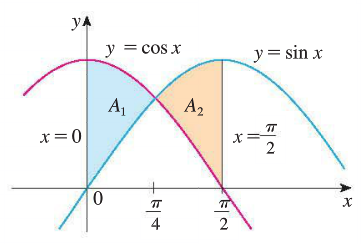
\includegraphics[scale=0.4]{6-1-pic7.png}\\

Some regions are best treated by regarding \underline{\hspace{0.3in}} as a function of \underline{\hspace{0.3in}}. If a region is bounded by curves with equations $x=f(y), x=g(y), y=c,$ and $y=d$, where $f$ and $g$ are continuous and $f(y)\geq g(y)$ for $c\leq y\leq d$, then its area is\\

\[\underline{\hspace{2in}} = \underline{\hspace{2in}}\]\\


where $x_R$ represents the right boundary and $x_L$ represents the left boundary of the region.
\indent

\[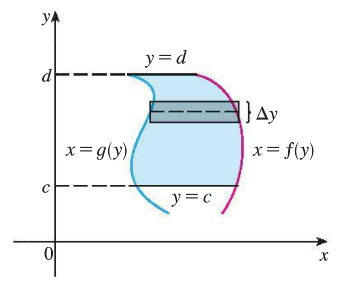
\includegraphics[scale=.4]{6-1-pic8.png} \hspace{1in} 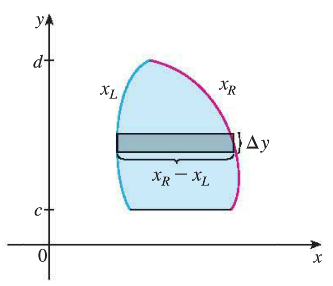
\includegraphics[scale=.4]{6-1-pic9.png}\]

\underline{Example 4}: Find the area enclosed by the line $y=x-1$ and the parabola $y^2 = 2x + 6$.\\

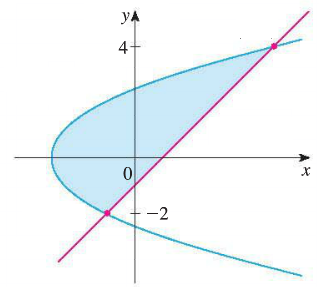
\includegraphics[scale=.4]{6-1-pic10.png} \hspace{0.4in} 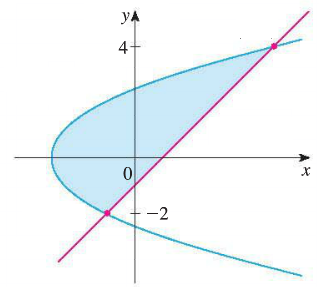
\includegraphics[scale=.4]{6-1-pic10.png}\\

\vspace{3in}

\newpage
\[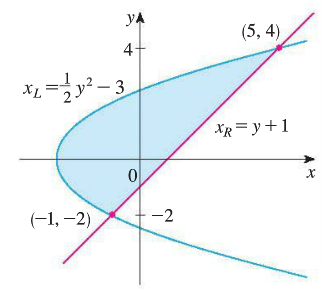
\includegraphics[scale=.45]{6-1-pic12.png} \hspace{1in} 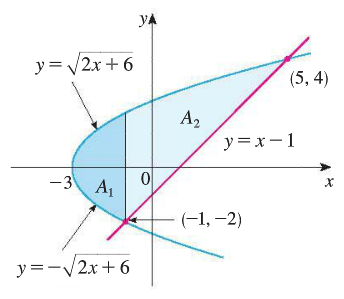
\includegraphics[scale=.45]{6-1-pic11.png}\]

\vspace{3in}

%----------------------------------------------------------------------------------------

\end{document}